\documentclass{below-ext}

\title{A standard for Home monitoring}

\numberofauthors{4}
\author{
  \vspace{-1.5em} 
  \alignauthor{
  	\textbf{Patrick Hendriks}\\
  	\email{patrick.hendriks@hva.nl}
  }
  \vfil
  \alignauthor{
  	\textbf{Mats Otten}\\
  	\email{mats.otten@hva.nl}
  }
  \vfil
  \alignauthor{
  	\textbf{Suzanne Peerdeman}\\
  	\email{suzanne.peerdeman@hva.nl}
  }
  \vfil
  \alignauthor{
  	\textbf{Glimworm IT BV}\\
  	\affaddr{Kattenburgerstraat 5}\\
  	\affaddr{1018 JA Amsterdam}\\
  }
}


\def\plaintitle{A standard for Home monitoring}
\def\plainauthor{Patrick Hendriks; Mats Otten; Suzanne Peerdeman}
\def\plainkeywords{Ambient environment; Elderly care; Healthcare technology}
\def\plaingeneralterms{Research}

\hypersetup{
  % Your metadata go here
  pdftitle={\plaintitle},
  pdfauthor={\plainauthor},  
  pdfkeywords={\plainkeywords},
  pdfsubject={\plaingeneralterms},
  % Quick access to color overriding:
  %citecolor=black,
  %linkcolor=black,
  %menucolor=black,
  %urlcolor=black,
}

\usepackage{graphicx}   % for EPS use the graphics package instead
\usepackage{balance}    % useful for balancing the last columns
\usepackage{bibspacing} % save vertical space in references
\usepackage{ragged2e} % alignment
\usepackage[utf8]{inputenc}
\usepackage[english]{babel}
\usepackage{lipsum}
\usepackage{epstopdf}
\usepackage{amssymb}
\usepackage{pifont}% http://ctan.org/pkg/pifont
\usepackage{float}
\usepackage{tikz}
\newcommand{\cmark}{\ding{51}}%
\newcommand{\xmark}{\ding{55}}%

\begin{document}

\maketitle

\begin{abstract}

The aging of the population of the Netherlands causes an ever growing need for solutions that enable the elderly to continue living independently for longer, while not putting their health and wellbeing at risk. Despite the wide range of products available, very few catch on. This leads to the question: how can we develop an accessible standard with which to add a layer of intelligence to the living environment? By conducting interviews and a focus group among the elderly residents of Stedeborgh, a living community in Grootebroek, the Netherlands, we found that this is largely because of a wrong view on what the target audience wants and needs; many consider their privacy invaded by existing systems, and feel that they do not have enough control over what is monitored and where the data ends up. As a response, we designed a prototype that is scalable and transparent, to add ambient intelligence to the living spaces of the target audience. The prototype was then deployed in the homes of the respondents. the results showed that rather than monitoring systems, a need exists for ambient environments that work together with and provide feedback to the user. This symbiosis allows for prolonged autonomy and peace of mind, as they user knows they are being looked out for, but do not feel scrutinized.

\end{abstract}

\keywords{\plainkeywords}
\category{H.5.m}{User studies (e.g., HCI)}{Miscellaneous}. 
%\terms{\plaingeneralterms}

% =============================================================================
\section{Introduction}
% =============================================================================
For the past several years, the changing demographics in the Netherlands has raised many concerns. The growing number of elderly people living alone and the question of how to care for the aging population causes immense pressure on the means available. Not only is there a risk of gradual and health decline, but also direct calamities such as falling incidents that go unnoticed. Annually, 1 in 180 people between the age of 55 to 64 receives emergency treatment after a fall in and around their home. This chance increases drastically up to 1 in 27 for 85+ \cite{seh}.  The growing demand for solutions has caused a  surge of technological developments aimed specifically at this target audience. However, even if a demand for ambient intelligence based systems such as these, the market does not quite seem to take off in the way that most developers hope for. Conduction of a focus groups among elderly people living independently has proven that the demand exists, yet is often not satisfied by what is currently on offer. Various systems target the caregivers of those that will actually be using the product, rather than the users themselves. It has become apparent that a large portion of the elderly population wishes to be respected in their autonomy, and take matters into their own hands.\cite{cbs_households}


\begin{figure}
\centering
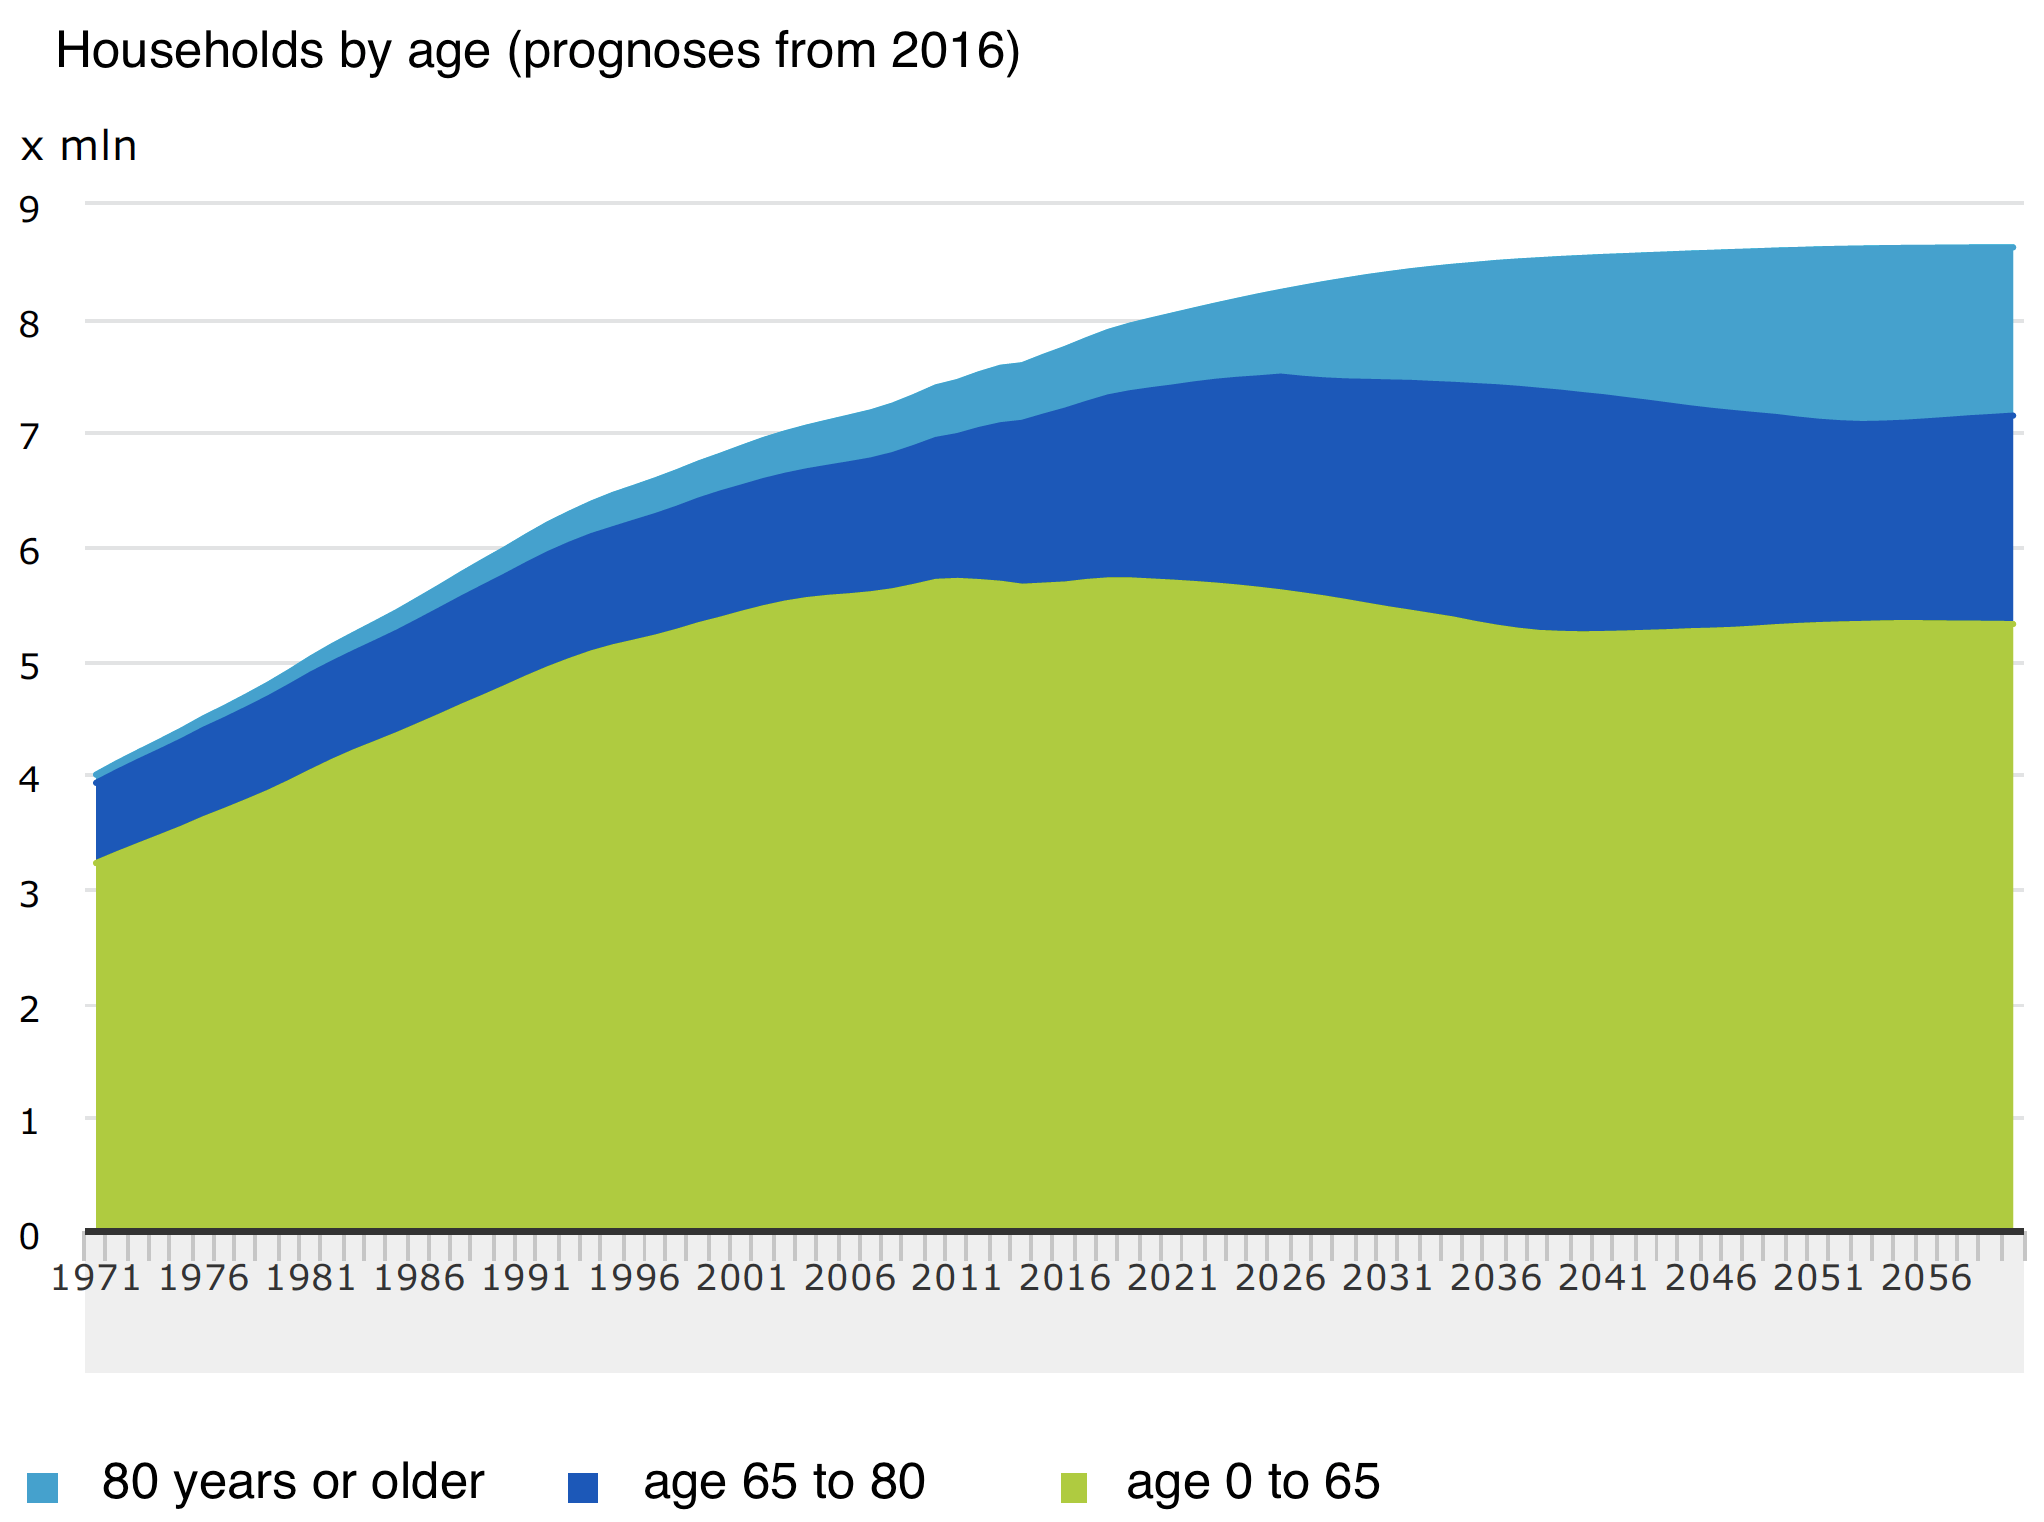
\includegraphics[width=0.5\textwidth]{cbs_household_age_report}
\caption[Translated graph]{Translated graph from CBS\footnotemark }
\label{fig:cbs}
\end{figure}
\footnotetext{Central bureau of statistics of the Netherlands}
The products available are also specifically targeted at an elderly audience, even though they would be able to cater a much more diverse group of users. Therefore, the goal of us is to lay the foundation for a portable living lab; a standard kit that can be used by anyone, even those with minimal technical experience, and that can be expanded upon by those that wish to do so.

A major part of this research was performed within Stedeborgh; a living community by the elderly for the elderly. Stedeborgh is a largely autonomous community, with residents aged 67 and up. For this paper several tests, a focus group and interviews were conducted among a group of 13 residents aged 65 or up, and their sentiments, routines and opinions have played a big part in the decisions that were made. Aside from Stedeborgh, this research was performed in collaboration with Amsterdam's Digital Life Centre's project BRAVO (led by Saskia Robben, 1 Apr 2016 - 1 Apr 2018) and Glimworm Information Technology (Adrian Blackwood). Collectively, the question we ask ourselves is: 
\begin{itemize}
\item"How can we develop an accessible standard with which to add a layer of intelligence to the living environment?" 
\end{itemize}

In this paper the focus will be on answering the aforementioned question, as well as answering several other questions:
\begin{itemize}
\item What monitoring systems are currently on the market, and what knowledge is available?
\item  What are the wishes of the target audience when it comes to improvement of living quality using technology?
\item How can the needs of the target audience be satisfied using technology?
\end{itemize}

This paper will begin with a report on literature and field studies performed to answer the first two of these questions. The third part will consist of reports on experiments and tests performed using prototypes. 


% =============================================================================
\section{Related Work}
% =============================================================================
%This section will focus on the state of the art technology as of this time (2017), as well as the current situation of Elderly care for senior citizens that are living independently or semi-independently in living groups. The first half of this section will illustrate how the care and national budget for this care are managed, what tools are frequently being used and what gaps are currently being encountered. Furthermore we will investigate how independent living groups have developed their own systems for keeping everyone healthy and autonomous. The second half of this section will briefly summarize the current state of the art technology, what advantages they offer the user, and what disadvantages are being encountered.

% =============================================================================
\subsection{Care for independent senior citizens}
% =============================================================================

A surprisingly big misconception when it comes to innovation aimed specifically at the elderly community, is that this is an audience that, as a whole, wants roughly the same thing; all share similar fears, weaknesses and requirements. In reality, however, there exists a myriad of different people all with different abilities and disabilities. Some are physical, such as bone atrophy, or mental, such as dementia or a combination of the two resulting from a stroke\cite{waag}. As of 2015, the government of the Netherlands has aimed to reform the long-term care for the elderly in such a way that more responsibility is given to the able citizen. This changes the nature of the long-term care program to that of a package of care and support which the active population, using their own resources, can call upon in order to maintain their autonomy and age with dignity\cite{langerzelfstandig}.

The policy in the Netherlands and other European countries is aimed towards enabling elderly citizens to grow old in their own homes and/or neighbourhoods (aging in place) by use of their own resources and a package for care and welfare facilities. \cite{thomas_blanchard} Despite the best efforts of fellow citizens and caregivers however, this method does not always suffice and, more importantly, does not give the loved ones of the elderly citizens in question peace of mind. This is where electronic monitoring systems get to play their part.


% =============================================================================
\subsection{Electronic monitoring for the elderly}
% =============================================================================
Electronic monitoring of elderly and/or vulnerable citizens is nothing new, there is a multitude of systems available that offer various degrees of support to the user. These vary from wearables that either monitor or aid the user, or both. Take for example the Lechal insoles: "Owned by the India-based company Ducere, Lechal offers a line of smart shoe inserts to help visually impaired wearers more easily navigate the world at large. These smart insoles provide directional assistance in the form of gentle vibrations and phone notifications, giving seniors a greater degree of independence. The associated app also allows for location sharing, letting you keep tabs on your loved one no matter where they are." \footnote{quoted from safewise.com} A simpler solution would be monitoring wearables similar to fitbits, which keep tabs on the user's heart rate and blood pressure, or simply a wearable alarm button which notify emergency services when pressed.

Of course, these are all relatively simple systems focusing on one particular element, but there are also various platforms available on market. In the spring of 2016 Philips introduced \textbf{CareSensus}, a sensor platform created in collaboration with Right At Home, one of America's biggest franchises for  home care services. This system was later deployed in the Netherlands by Cordaan, a major home care institution in Amsterdam, to aid people suffering from dementia. CareSensus proved the potential succes of deploying various sensors in the living environment for health monitoring. Another solution is Sensara. Placing second in 2014's Game Changer Award, Sensara is another monitoring system focusing specifically on users in early to advanced stages of dementia. The system keeps track of the user's activity; specifically whether or not the user gets out of bed in the morning, how often the user leaves their house and whether or not they return. In case of an emergency, mantle care will be alerted. Care@Home by Essence offers a line of products that include voice and fall recognition, and send an alert out to emergency services if the system deems it necessary.Another system, Livind, analyses the user's behaviour and will send a text message to mantle care in case of deviation. 

% =============================================================================
\section{Pre-design research}
% =============================================================================

\subsection{Stedeborgh}

Before the creation of the prototype we visited Stedeborgh, an independent living community for the elderly, to gather some first hand insights and information. Stedeborgh is an independent living community situated in Grootebroek, the Netherlands.  It is not your standard nursing home; it is for the elderly, by the elderly. The residents live alone or in couples in fully fledged apartments, meaning each apartment has its own kitchen and bathroom as well. The apartments face to the inside of the complex, rather than to the outside, and are connected by an indoor garden featuring tropical foliage and equally tropical temperatures \ref{fig:stedeborgh}. on the ground floor is a large entertainment hall which is perfect for get-togethers, and a cafeteria for special events. The complex is surrounded by a lovely community garden. What makes Stedeborgh stand out most, however, is the way in which the residents look out for each other.\\
\vspace{0.2cm}
\begin{figure}
\centering
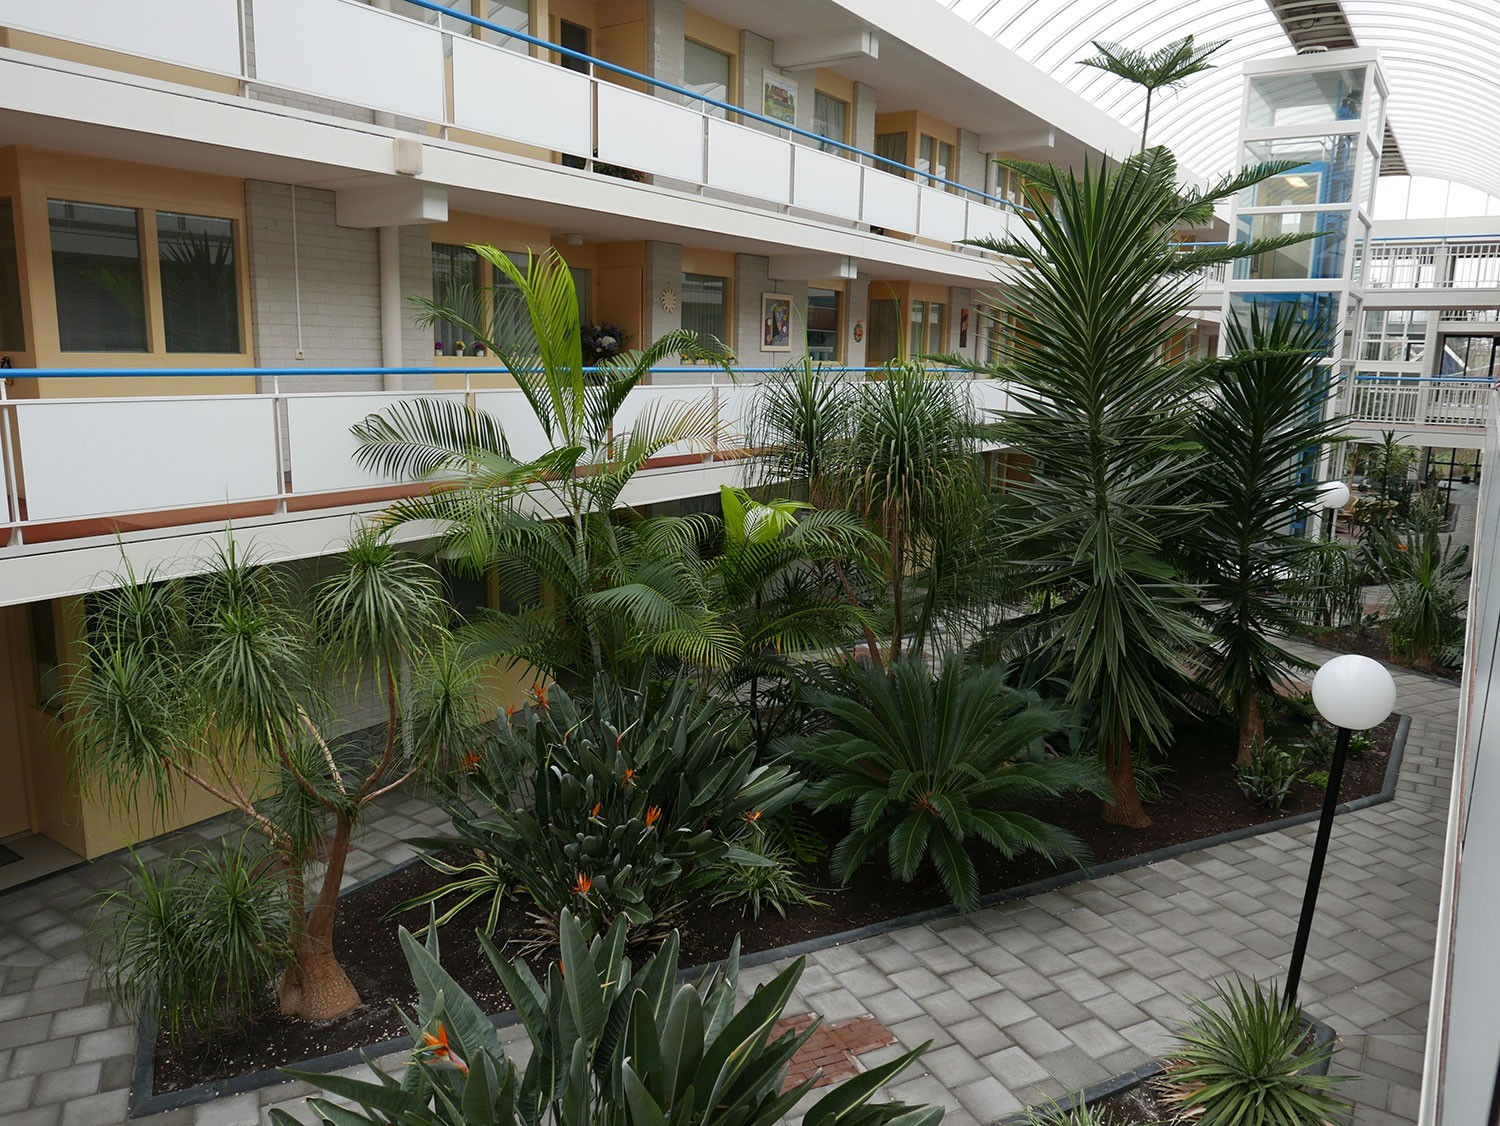
\includegraphics[width=0.45\textwidth]{stedeborgh}
\caption{Stedeborgh courtyard}
\label{fig:stedeborgh}
\end{figure}

\subsection{Systems}
The community is maintained by its residents, which means that everyone has a task and responsibilities within the community. A number of systems has been put in place to ensure the safety and wellbeing of the residents. The system that inspired us most was the "asleep/ awake" system. Every apartment has a sign on the door with a sun on one side, and a moon on the other. This sign is turned accordingly whenever the residents go to sleep, and whenever they wake up in the morning. The residents take weekly shifts in which they pass by all the doors in the evening and first thing in the morning. If a sign has not been turned appropriately this could be an indication that something has gone wrong, and the appointed member of the community will check up on their peer immediately. This method, however simple it may be, has proven to be very effective in solving one of the major concerns when it comes to the safety of elderly people living alone; injury by fall. Countless accounts exist of elderly people falling down within their own homes and being unable to get up. In the worst of these cases, the victim may spend days incapacitated on the ground without anyone coming to their aid, sometimes even with death as a result. The system in Stedeborgh ensures that the residents, at the very least, are not without aid for longer than eight hours. 

\subsection{Stedeborgh as a target audience}
As we were inspired by this community's way of life, and the living quality of its residents, we decided to make the residents of Stedeborgh our main target audience, and design our use cases for this research around them. We were curious about their stance on the use of technology for health-monitoring, and what would make such a system attractive to them, both as individuals, and as a community. We made the decision to conduct a focus group among those that were interested in our research.

% =============================================================================
\section{Focus group}
% =============================================================================

As part of our research, we conducted a focus group at Stedeborgh among a group of volunteers. The group met in the cafeteria where they were provided with coffee, tea and sweets. We strove to keep the atmosphere as casual and relaxed as possible, to encourage the participants to speak freely and openly about the subject. The participants were introduced to us and, surprisingly enough, did not require too much explanation. Whereas most of the performed desk research concluded that the elderly population of the Netherlands was near phobic of technology, the residents of Stedeborgh proved the contrary: many were already familiar with several systems on market today, and some even owned their own.

\subsection{Stigma}
\label{ref:alarm_button}
 One of the older participants, a lady nearing her 90's, told the group she always had her alarm button with her, attached to her walker. The woman had trouble walking due to bone atrophy, but was still living independently. When asked about the stigma devices such as these carry, she responded casually: "I am an elderly woman, at my age no one should feel ashamed about carrying a device that helps them in case of emergency. You all have your cell phones too, don't you?" She also told us that the device has thus far helped her maintain her autonomy to quite an extent. She has not yet had a falling incident, but she is very well aware of the fact that she is at risk. The alarm button gives her a sense of security that has given her the confidence to continue doing the things she does. Because if she were to fall, she would be able to immediately call for aid. The majority, if not all of the respondents, agreed with her.

\subsection{Monitoring}
During this first discussion the respondents expressed a clear wish for products such as the one we aimed to develop. We were told that commercial parties had come by several times already to offer their services and products. When asked for the main reason why there was never an investment in these products, the respondents had some very clear explanations. Stedeborgh is an independent community run mainly by its residents, and it simply couldn't afford to spend up to thousands of euros on products that piqued their interest, but had not yet proven their worth to the community's satisfaction. More importantly, however, the respondents stressed the fact that the systems often lacked transparency. Many of the presented solutions made use of cameras, which aroused a sense of unease in the users. An issue that had already been addressed in various papers, including "Ambient Monitoring from an Elderly-Centred Design Perspective: What, Who and How" \cite{Kanis:2011:AME:2177525.2177579}.Where the respondents expressed specific concerns about not only their own privacy, but that of potential house guests as well.

One man told us that even though he was ensured that the visual data captured would be analyzed by algorithms rather than people, this did not take away the feeling of being watched. "The word algorithm doesn't give me any idea of what is happening inside," he said half jokingly. "If you tell me an algorithm is analyzing my video feed, you might as well just tell me a midget or a ghost is watching me." Many of the respondents agreed that the systems were not transparent enough, and not only because they were described using terminology which did not resonate with them. Some even went as far as to admit the way the systems were designed made them feel like children being watched. % Te lange quote hieronder volgens Mats 
"Most of these systems are made in such a way that they will provide reports about your well being to a caretaker or a doctor. I do not want that. If I am feeling under the weather I would much rather have my daughter calling me to see if I am doing ok than have a nurse rush in to usher me out of bed because I am 'not getting enough exercise'," one of the relatively younger women stated. 

\begin{figure}
\centering
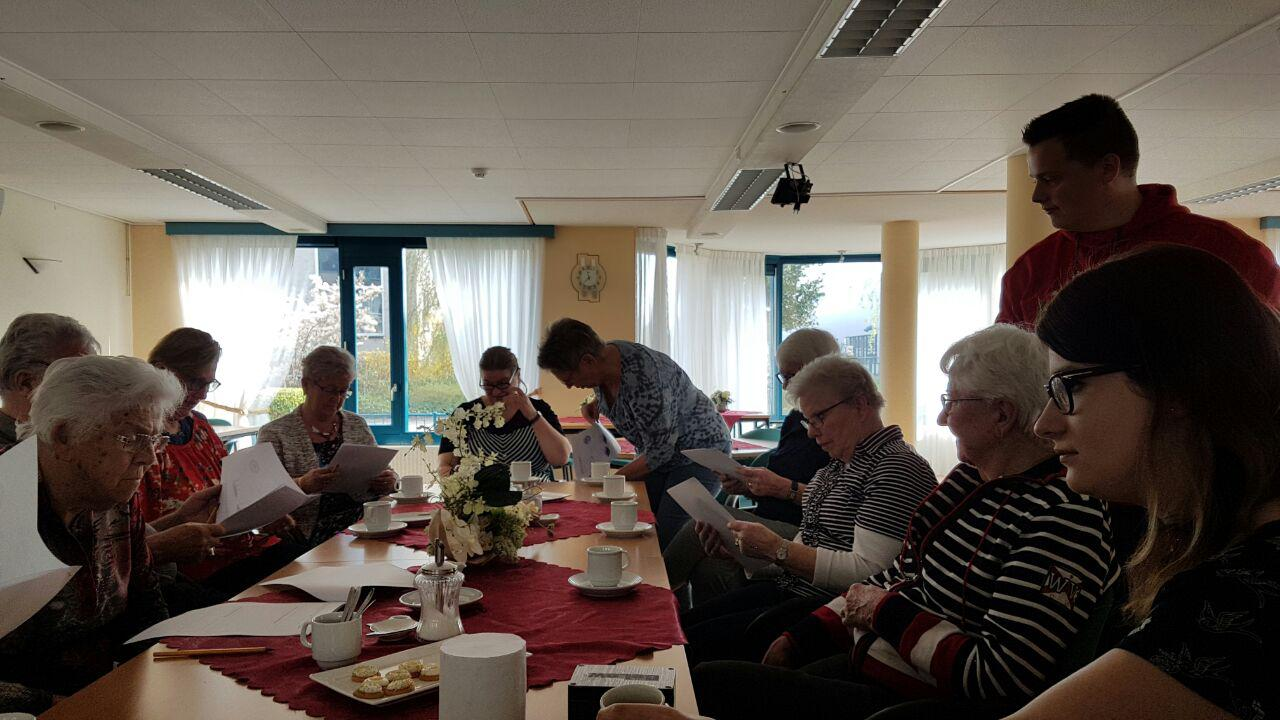
\includegraphics[width=0.5\textwidth]{interview}
\caption{Interview Group}
\label{fig:interview}
\end{figure}

%==============================================================================
\section{Technology}
%==============================================================================
Over the past decades technology has changed the face of domestic life. Devices are becoming, smaller, faster and more economical. They are ubiquitous and omnipresent, and this provides a myriad of new opportunities. About twenty years ago a pocket phone was a novelty reserved only for the privileged, now most western people cannot live without their smartphone. Not only that, but these smartphones carry an array of sensors that could only be found in laboratories less than a generation ago. This has opened the door to more readily available, advanced and accessible technology for health care and wellbeing.

\subsection{Technology in the prototype}

For our field research we designed and created a prototype to be deployed in the homes of our respondents. The goal for the prototype was to make it portable and scalable. We designed the system hierarchy in such a way that each individual system would consist of a single gateway with cloud connectivity to funnel the data gathered within a home into a single database. This gateway  in turn is able to receive data from several sensor 'nodes' that can be added or subtracted at will and are placed throughout the user's home. 
 
The advance of technology does not move equally fast everywhere, however. It quickly became apparent that when designing a system that is required to push the data it gathers to a central point one cannot always rely on the Internet as a transmission medium. Many of the nursing homes, living communities or independent respondents that were contacted during the pre-design phase did not have an Internet connection in every home, or none at all. This led us to believe that it would be a safe bet to incorporate the IoT\footnote{Internet of Things} LoRa\footnote{Low power Radio} technologies into the prototype to ensure that it would not malfunction due to a poor connection. As of 2016, KPN offers complete LoRa connectivity throughout the Netherlands, and this coverage will only continue to grow. LoRa is able to transmit messages over distances of up to 10 KM whithout a continuous or heavy duty power source. LoRa does, however, offer limited message size and frequency. 


Because of LoRa's restrictions when it comes to message frequency, only the gateway uses LoRa for communication. The nodes communicate with the gateway through Bluetooth low energy. This relatively new incarnation of Bluetooth consumes minimal power, which is of the utmost importance because the nodes are battery powered. To conserve energy the nodes remain in deep sleep mode until they receive input from one of their  'trigger' sensors. These are the sensors that indicate that the user is in the room and that data should be recorded. the node will then broadcast its acquired data to the gateway, which filters it and prepares it for LoRa transmission. These complex tasks are not performed by the nodes in order to conserve energy.  

\begin{figure}
\centering
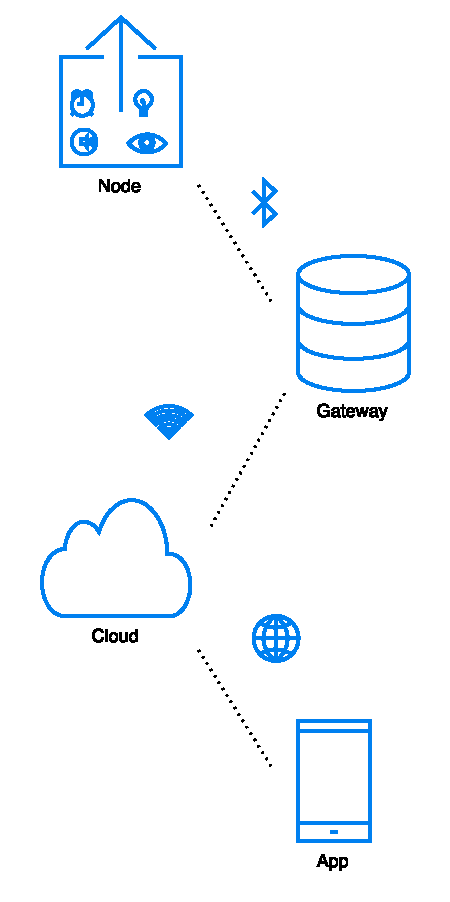
\includegraphics[scale=0.6]{dataproces.pdf}
\caption{Schematic of the data collection process}
\label{fig:process}
\end{figure}

\subsection{Open standards}

By creating not only a product, but an example of a product standard, we would like to enable developers and hobbyists to engage with the product and expand upon the technology and possibilities. The grove shield plays a big part in this, as it allows for up to 13 sensor modules and a BLE\footnote{Bluetooth Low Energy} to be connected to a node controller. The underlying code was designed with this in mind; only the BLE module has a set position. All other sensor positions are interchangeable. Because of this structure, one can easily add and remove sensors without any prior programming experience. This method also allows for new devices to be added to the network without revision of the existing system. Imagine, for example, a pill case that sends out a signal whenever opened; such a gadget could mean a great improvement to the wellbeing of the user, and it could be added on a whim. 

Designing a product in this open manner requires a carefully thought out structure. In our opinion, there should be two versions of the same product: a ready made, and a DIY\footnote{Do it yourself} variety. This means that the base system would both be available as a product, and as a kit. This kit especially, would not only be fit for use in the homes of elderly users, but can easily be transformed into a portable living lab; a way to quickly and efficiently add intelligence to any space. This could be especially useful not only for those wishing to create an ambient space for personal use, but to students as well. The added value this could possibly grant future studies performed at the digital life centre adds an interesting new dimension to the whole


\subsection{Goal}

The ultimate goal when developing the prototype, is to see whether or not solutions that are currently present in the form of expensive and closed commercial technologies, can be molded into the shape of a community based platform. During this proces we will have to be constantly aware of the fact that specialized care or technologies will always remain necessary in many cases. However, over the past years more and more platforms of increasing technological prowess such as Arduino, Raspberry Pi et cetera have become available to the public. These platforms come with an array of sensors capable of measuring everything from sound, to temperature, to light. These sensors are relatively accurate, but often do lack the reliability to truly gain knowledge from individual measurements. For this, machine based learning can offer the solution. Studies have explored the possibilities of linking the motor score of AMPS\footnote{Assessment of motor and process skills} to the sensor data using linear regression\cite{robben2012grandma}. Through machine based learning correlations, patterns and deviations from these two can be detected and eventually add valuable layers to the gathered data. The platform offers a method to gather large amounts of data. With the help of specialists, machine based learning and continuation of research we hope to eventually shape this data into information, knowledge, and finally wisdom (Figure \ref{fig:dikw}). Once the wisdom layer is reached, it becomes possible to not only respond to calamities, but prevent them altogether. This way, the final product will unburden the caregivers and the care budget, and  be shaped after the wishes of the target audience  while still preventing human error through its self-learning capabilities.

\begin{figure}
\centering
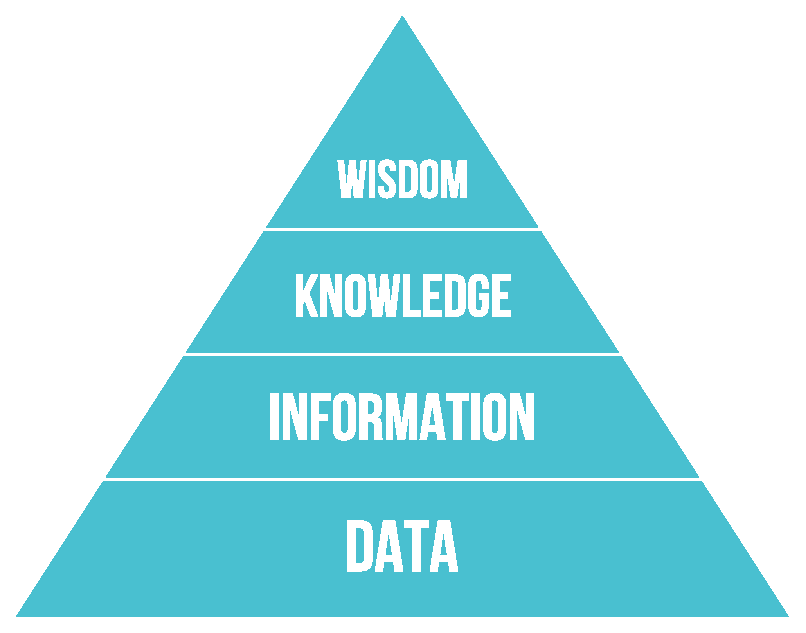
\includegraphics[width=0.4\textwidth]{dikw}
\caption{Data Information Knowledge Wisdom model}
\label{fig:dikw}
\end{figure}

% =============================================================================
\section{Practical testing}
% =============================================================================
The prototype was focused around scalability, meaning that sensors could quickly be added and removed without the need for tools. The main controller used, the Sodaq Autonomo, and its compatible Grove shield enabled this. The Grove modules created by Sodaq made it possible to entertain a plug-and-play approach, so that the prototype could we adjusted whenever needed. 
\begin{figure}
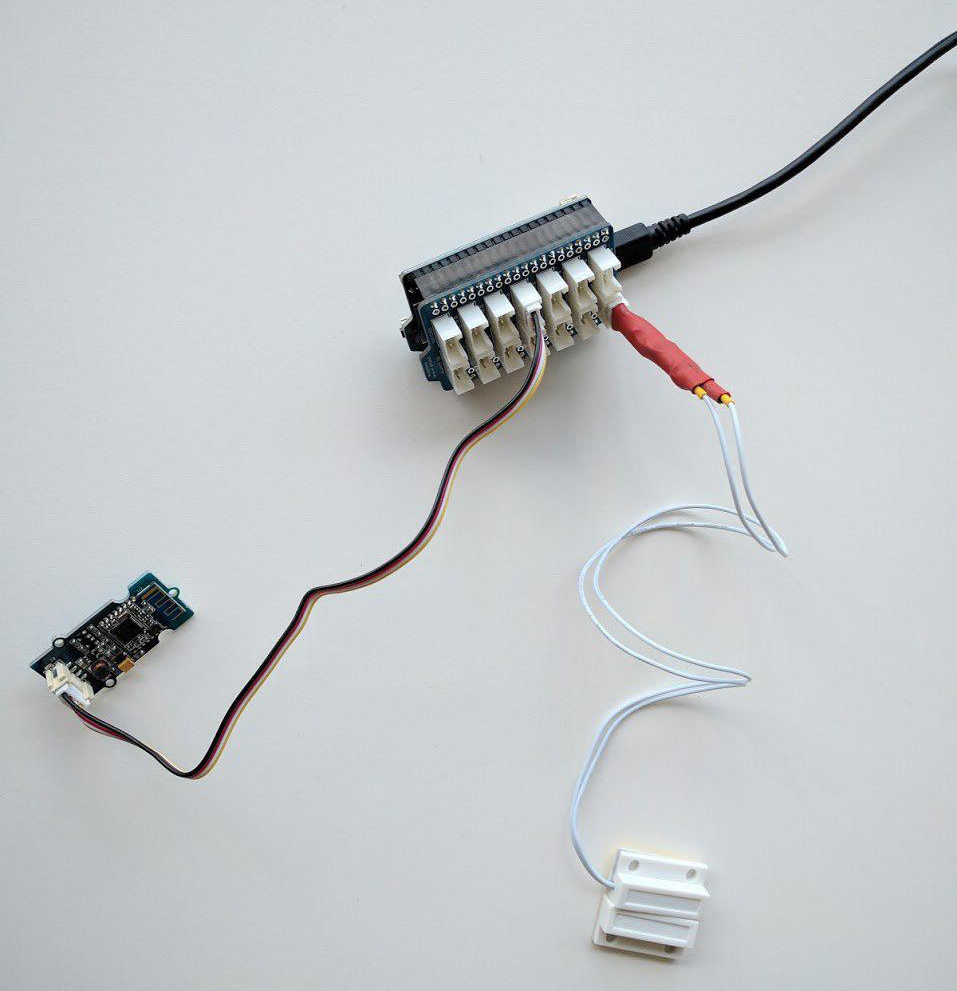
\includegraphics[width=0.5\textwidth]{sodaq}
\caption{Sodaq prototype}
\label{fig:sodaq}
\end{figure}
sensor technology was kept relatively simple. The nodes were equipped with a passive infrared sensor, a light sensor, a temperature sensor, and an optional magnetic door sensor to monitor the opening of doors and windows. Each respondent was then supplied with a single gateway and two nodes that were to be strategically placed in their living area. The group of respondents consisted of elderly couples, single elderly people, and students. During this phase, emphasis was on the functionality of the system, and making the data available to the users. 

\subsection{Room monitoring}

\begin{figure}
\begin{tikzpicture}
\node[inner sep=0pt] (russell) at (0,0)
    {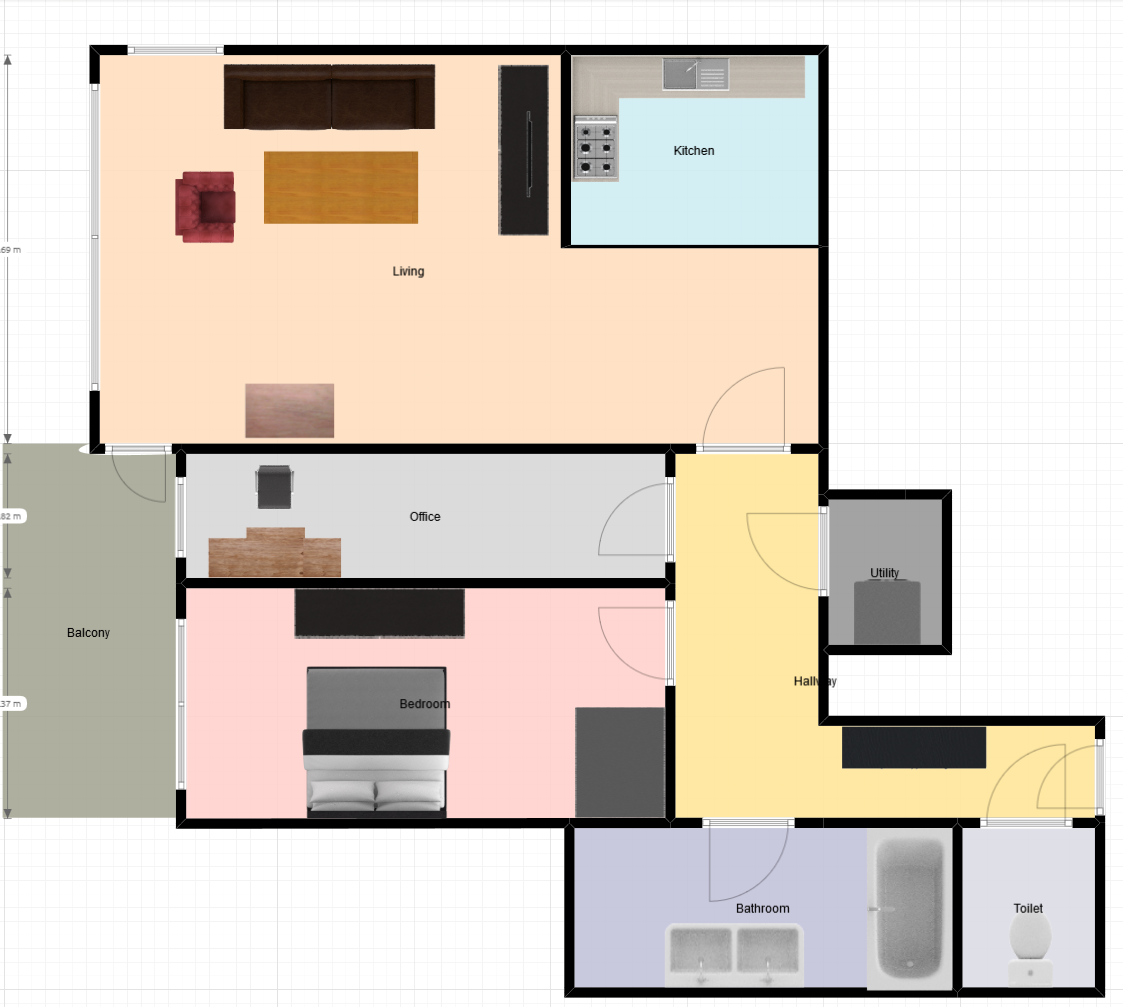
\includegraphics[width=0.5\textwidth]{floorplan.png}};
\draw[fill=purple] (1.5,0.6) circle (0.3cm);
\draw[fill=blue] (-3.1,2.9) circle (0.3cm);
\draw[fill=purple] (3.5,-2.6) circle (0.3cm);
\draw[fill=purple] (-2.5,-1.6) circle (0.3cm);
\draw[fill=purple] (-3,-4) circle (0.3cm);
\draw[fill=blue] (-3,-4.7) circle (0.3cm);
\node[draw,text width=1.2cm] at (-1.5,-4.7) {Gateway};
\node[draw,text width=1.2cm] at (-1.5,-4) {Sensor};
\end{tikzpicture}
\caption{Floorplan of field-test}
\label{fig:floorplan}
\end{figure}
In the home of one of the respondents three sensor nodes were placed for data acquisition. The nodes were placed strategically to gather the most relevant data. Figure \ref{fig:floorplan} shows the floor plan of the residence in question, as well as where the sensors were placed.

\subsection{Sensor data}
One of the main questions concerning the sensor nodes was the battery life, and whether it would be sufficient to allow for prolonged periods of data acquisition. Temperature was measured at a 30 second interval, whereas movement and the opening of doors was measured based on triggers. As the trigger-based sensor nodes will always require less power because they spend the majority of the time in deep sleep modus, the temperature node was used in order to get a realistic view on battery life. Figure  \ref{fig:temp} shows data gathered between 24-5-2017 00:00 and 24-5-2017 12:00. We began measuring on 22-5-2017 with a battery capacity of 2300mah. On 26-5-2017, this was down to 2088mAh, meaning that the system had used 212 mAh over the span of four days, approximating at a usage of  $\pm$ 53 mAh per day.

\begin{figure}
\centering
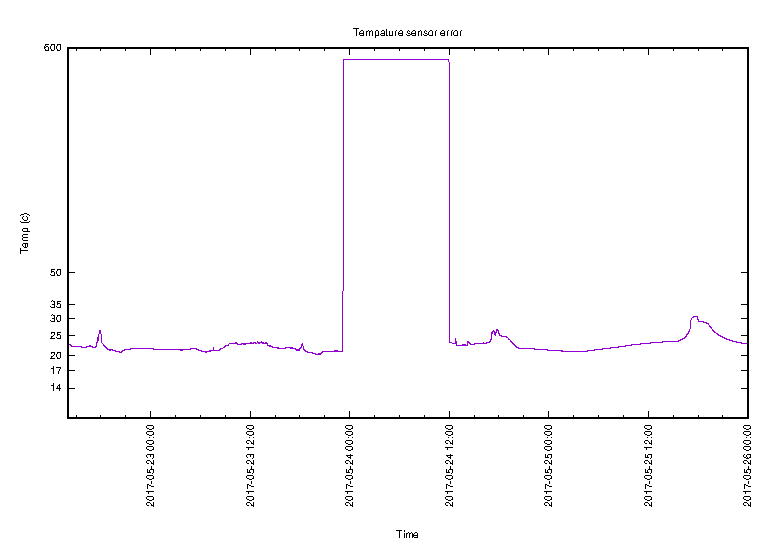
\includegraphics[width=0.5\textwidth]{temperror}
\caption{Temperature graph with error}
\label{fig:temperror}
\end{figure}

In  Figure \ref{fig:temperror} we can see there is a large spike caused by a malfunction in the sensor. Because of this spike, nearly all details in the figure are lost.

\begin{figure}
\centering
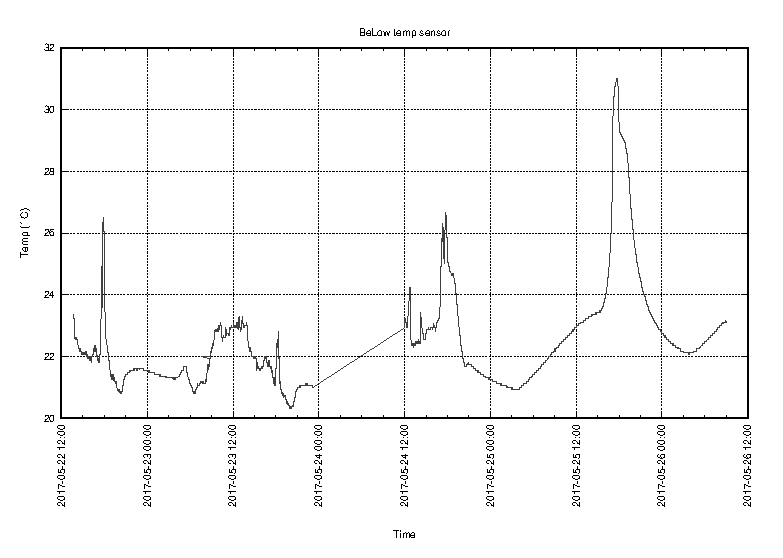
\includegraphics[width=0.5\textwidth]{graph}
\caption{Temperature graph}
\label{fig:temp}
\end{figure}

Figure  \ref{fig:temp} contains the same graph, but with the spike filtered out. We have done this by filtering out all unrealistic temperature in- and decreases. We were unable to discover what caused the error. Strangely, there was only this one spike, while one would expect the sensor to malfunction more than once in a case like this.

\begin{figure}
\centering
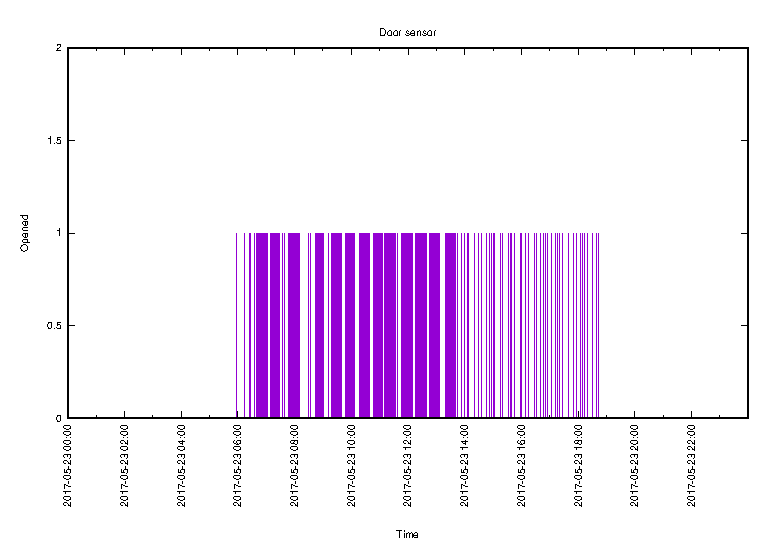
\includegraphics[width=0.5\textwidth]{doorsensor}
\caption{Door sensor recordings}
\label{fig:doorsensor}
\end{figure}

Finally, Figure \ref{fig:doorsensor} shows data from a door sensor linked to one of the doors within one of the buildings of the Amsterdam University of Applied Sciences, and clearly shows the activity in that particular hallway throughout the day. This is an essential tool for the monitoring of in-home activity, as it serves as a checkpoint that the user passes through during their daily routines.

%==============================================================================
\section{Discussion}
%==============================================================================
An important next step once the data has been gathered, is creating a layer of wisdom. This is done through prolonged periods of data acquisition, and adding context to them based on patterns uncovered by means of machine learning and thorough analysis so that the data may be well understood, and predictions may be done based off this understanding. More efforts should be put into designing systems in such a way that they can be blended into the living space, and customized according to the user's wishes. Furthermore, our respondents stressed the importance of feedback. This is what really creates interaction with the environment because it may not only be used to keep the user up to date, but also to stimulate the user to perform certain actions and maintain daily rituals that are beneficial for their health and wellbeing, as well as recognizing early symptoms of otherwise serious conditions.
%==============================================================================
\section{Conclusion}
%==============================================================================
As the demographics in the Netherlands continue to change, each generation finds itself responsible for the wellbeing of the one before it. The rise of technology may offer some relief, provided it is done in the right way. The rising demand for systems supporting the elderly in their autonomy and wellbeing, has caused many of the companies answering this demand to lose sight of the wishes of the target audience itself. The systems are shaped after the needs and wishes of those giving care to the elderly, and focus on a group of people with diminished cognitive abilities as a result of dementia and other neurological disabilities. In the pursuit of unburdening those that supply care, the needs of those that wish to receive care are foregone. Within the population, there exists a large group that does not need to be constantly looked after, but instead wishes for a system that will support them, and assist them in their time of need. Rather than a monitoring system, focus needs to be on creating an ambient environment that will not only watch and alert, but interact with the user and add intelligence to the living environment. This will in time create a symbiosis between man and machine that allows the user to remain independent for as long as possible, without the fear of having a decline in health or a calamity go unnoticed.

%==============================================================================
\section{Acknowledgements}
%==============================================================================

This paper is the result of a collaboration with Glimworm IT, most notably Adrian K. Blackwood and Paul Manwaring. Furthermore we would like to thank the residents of Stedeborgh for their time and effort during the interviews and experiments, and opening up their homes to us. Finally, we would like to thank Saskia Robben and Aukje de Vrijer of research team CREATE-IT, Amsterdam University of Applied Sciences for their support, input and coaching.

\nocite{Kanis:2013:SMH:2534504.2534526}
\nocite{Robben:2013:LRA:2534504.2534555}
\nocite{langerzelfstandig}
\nocite{NaitAicha:2013:LYG:2494091.2497283}
\nocite{stedeborgh}
\nocite{Nehmer:2006:LAS:1134285.1134293}
\balance
\bibliographystyle{acm-sigchi}
\bibliography{refs}
\end{document}
